\documentclass[a4paper, 11pt, twoside]{article}

\usepackage[utf8]{inputenc}
\usepackage[ngerman]{babel}
\usepackage[T1]{fontenc}

\usepackage{graphicx}

\usepackage[citecolor = black,colorlinks=true,linkcolor=black,urlcolor=black]{hyperref}

\author{Horst}
\title{Unser tolles LUG-Dokument}
\date{7. März 2037}

\hyphenation{ab-spei-chern}

\begin{document}

\maketitle

\newpage

\tableofcontents
\listoffigures


\newpage

\pagenumbering{alph}


\section{ich bin neu}

\begin{figure}[h]
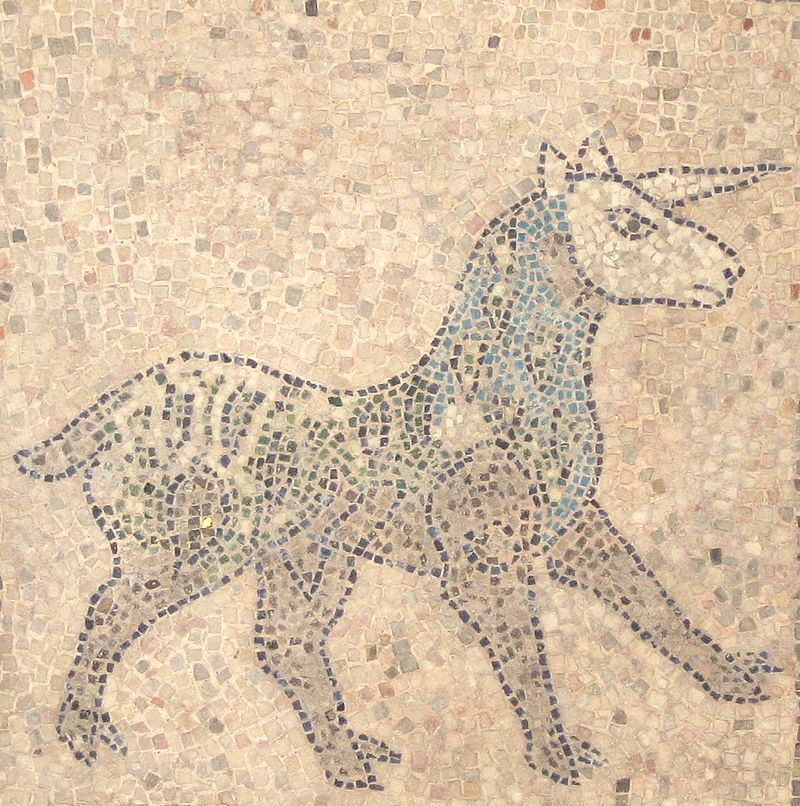
\includegraphics[width=\textwidth]{einhorn.jpg}
\caption[Was anderes]{Mein Einhornbild}
\label{fig:Einhorn}
\end{figure}

\section{Tabellenbeispiel}

\begin{table}[h]
\begin{tabular}{|l|c|r|}
\hline
e & a & u\\
\hline
Ich sollte linksbündig sein und so lang, dass ich eigentlich nicht auf eine Zeile passen kann.& Ich nicht & Ich bin rechtsbündig! \\
\hline
\end{tabular}
\end{table}

\section{Hallo LUG!}
\label{lug}
Ich begrüße die Linux User Group in der Rabryka\footnote{Isdkjfh sjkdhf kdjsfh ksjdfh ksjdf kjsdfh kjsdhf kjsdf kjsdfh kjsdfh kjsdfh jsdf kjsdfh kjsdfh jksdf hsdjkfch bin die tolle Fußnote}!


$HUI = \int 2x$

\[ \int 2abx \pi \frac{1 \delta y}{2}\]

\section{sdfjhsdfk}

\begin{itemize}
\item Stichpunkt
\item[i] 42
\end{itemize}

\begin{enumerate}
\item Test 
\item[] noch ein TEst
\item und noch einer!
\end{enumerate}

\begin{description}
\item[Mein Zeugs] Das beschreibt beim Zeugs! Wie in Bild \ref{fig:Einhorn} zu sehen ist.
\item[Ein etwas längerer Punkt] Aber die Beschreibung ergibt auch nicht viel mehr Sinn!
\end{description}

\section{Neuer Abschnitt}

\textit{sdj} fhkjsdfhkjsdfh \tiny huiiiii





\large
large

\Large
Large sdjfskhdf dsjkf hkjsdfh ksjd fhksdf hdskjfh skdjfh ksdjfh ksjdf   dsklfjdslkfj lsdkfj lksdfj lksdfj lksdfj lskdfj klsdjf \\ lsdjf lksdjf lskdjf lskdfj lksdjf lksdjf lskdfj lksdjf lskdjf lksdjf lksdfj lskdfj lskdfj lksdfj lskdfj lskdfj dsfhksjdf hkj Ich hab das schon in Kapitel \ref{lug} gesagt!
\newpage

\LARGE
\textit{\textbf{LARGE}}

\normalsize

 \textbf{auch das wird fett} kjdshf kjdsf 

%https://github.com/sanguinik

udfhkjsdfhsjdf 
kjdsfkdsjfh 
\subsection{Untergeordnet}



%Ich nehm die Caprese!
\end{document}
